\documentclass[letterpaper]{article}
\usepackage[margin=1in]{geometry}
\usepackage[utf8]{inputenc}
\usepackage{textcomp}
\usepackage{amssymb}
\usepackage{natbib}
\usepackage{graphicx}
\usepackage{gensymb}
\usepackage{amsthm, amsmath, mathtools}
\usepackage[dvipsnames]{xcolor}
\usepackage{enumerate}
\usepackage{mdframed}
\usepackage[most]{tcolorbox}
\usepackage{csquotes}
% https://tex.stackexchange.com/questions/13506/how-to-continue-the-framed-text-box-on-multiple-pages

\tcbuselibrary{theorems}

\newcommand{\R}{\mathbb{R}}
\newcommand{\Z}{\mathbb{Z}}
\newcommand{\N}{\mathbb{N}}
\newcommand{\Q}{\mathbb{Q}}
\newcommand{\C}{\mathbb{C}}
\newcommand{\code}[1]{\texttt{#1}}
\newcommand{\mdiamond}{$\diamondsuit$}
\newcommand{\PowerSet}{\mathcal{P}}
\newcommand{\Mod}[1]{\ (\mathrm{mod}\ #1)}
\DeclareMathOperator{\lcm}{lcm}

%\newtheorem*{theorem}{Theorem}
%\newtheorem*{definition}{Definition}
%\newtheorem*{corollary}{Corollary}
%\newtheorem*{lemma}{Lemma}
\newtheorem*{proposition}{Proposition}


\newtcbtheorem[number within=section]{theorem}{Theorem}
{colback=green!5,colframe=green!35!black,fonttitle=\bfseries}{th}

\newtcbtheorem[number within=section]{definition}{Definition}
{colback=blue!5,colframe=blue!35!black,fonttitle=\bfseries}{def}

\newtcbtheorem[number within=section]{corollary}{Corollary}
{colback=yellow!5,colframe=yellow!35!black,fonttitle=\bfseries}{cor}

\newtcbtheorem[number within=section]{lemma}{Lemma}
{colback=red!5,colframe=red!35!black,fonttitle=\bfseries}{lem}

\newtcbtheorem[number within=section]{example}{Example}
{colback=white!5,colframe=white!35!black,fonttitle=\bfseries}{def}

\newtcbtheorem[number within=section]{note}{Important Note}{
        enhanced,
        sharp corners,
        attach boxed title to top left={
            xshift=-1mm,
            yshift=-5mm,
            yshifttext=-1mm
        },
        top=1.5em,
        colback=white,
        colframe=black,
        fonttitle=\bfseries,
        boxed title style={
            sharp corners,
            size=small,
            colback=red!75!black,
            colframe=red!75!black,
        } 
    }{impnote}
\usepackage[utf8]{inputenc}
\usepackage[english]{babel}
\usepackage{fancyhdr}
\usepackage[hidelinks]{hyperref}

\pagestyle{fancy}
\fancyhf{}
\rhead{CSE 105}
\chead{Monday, January 10, 2022}
\lhead{Lecture 3}
\rfoot{\thepage}

\setlength{\parindent}{0pt}

\begin{document}

\section{Complementation}
\begin{theorem}{Complementation}{}
    If $A$ is a regular language over $\{0, 1\}^*$, then so is its complement. 
\end{theorem}
\textbf{Remarks:}
\begin{itemize}
    \item This is essentially the same thing as saying that the class of regular languages is closed under complementation.
    \item How do we apply this? Let $A$ be a regular language. Then, there is a DFA $M = (Q, \Sigma, \delta, q_0, F)$ such that $L(M) = A$. We want to build a DFA $M'$ whose language is $\overline{A}$. Define: 
    \[M' = (Q, \Sigma, \delta, q_0, Q \setminus F)\]
\end{itemize}

\begin{proposition}
    $M'$ accepts $A^c$.
\end{proposition}

\begin{mdframed}[]
    \begin{proof}
        Because $M$ accepts $A$, we define $A$ to be: 
        \[A = \{w \mid M \text{ accepts } w\} = \{w \mid \delta^{*}(q_0, w) \in F\}\]
        Recall that $\delta^{*}(q, w)$ is the state reached from $q$ after reading the word $w$. Taking the complement of $A$, we have: 
        \[A^c = \{w \mid w \notin A\} = \{w \mid \delta^{*}(q_0, w) \notin F\} = \{w \mid \delta^{*}(q_0, w) \in Q \setminus F\}\]
        So, $M'$ accepts $A^c$. 
    \end{proof}
\end{mdframed}

% temp solution for no warnings
\newpage 
\subsection{Example 1: Building DFA}
Construct a DFA that recognizes $\{w \mid w \text{ contains the substring baba}\}$.

\begin{mdframed}[]
    \begin{center}
        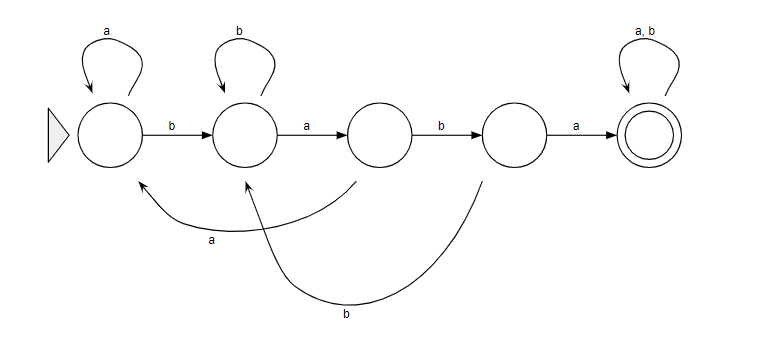
\includegraphics[scale=0.7]{../assets/baba_state.png}
    \end{center}
\end{mdframed}

\subsection{Example 2: Building DFA}
Construct a DFA that recognizes $\{w \mid w \text{ doesn't contain the substring baba}\}$.

\begin{mdframed}[]
    \begin{center}
        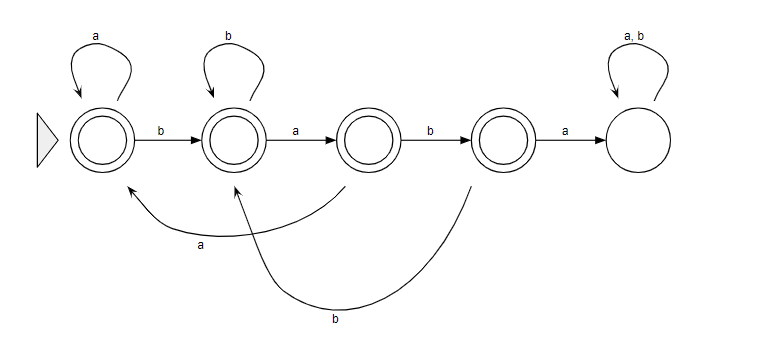
\includegraphics[scale=0.7]{../assets/not_baba_state.png}
    \end{center}
\end{mdframed}

\newpage
\section{The Regular Operations}
In arithmetic, the basic objects are numbers and the tools are operations for manipulating them (e.g. $+$ or $\times$). In the theory of computation, the objects are languages and the tools include operations designed for manipulating them. We call these \textbf{regular operations}.

\begin{definition}{}{}
    Let $A$ and $B$ be languages. We define the regular operations \textbf{union}, \textbf{concatenation}, and \textbf{star} as follows: 
    \begin{itemize}
        \item \textbf{Union:} $A \cup B = \{x \mid x \in A \text{ or } x \in B\}$.
        \item \textbf{Concatenation:} $A \circ B = \{xy \mid x \in A \text{ and } y \in B\}$
        \item \textbf{(Kleene) Star:} $A^* = \{x_1 x_2 \dots x_k \mid k \geq 0 \text{ and each } x_i \in A\}$
    \end{itemize}
\end{definition}
\textbf{Remarks:}
\begin{itemize}
    \item The union operation simply takes all strings in both $A$ and $B$ and puts them together into one language.
    \item The concatenation operation attaches a string from $A$ in front of a string from $B$ in \emph{all possible ways to get the strings in the new language}.
    \item The star operation attaches any number of strings in $A$ together to get a string in the new language. Note that \emph{any number} includes 0, so the empty string $\epsilon$ is always in $A^*$.
\end{itemize}
Note that we can prove the union operation today, but we cannot prove the concatenation or star operators until later.

\subsection{Union}
\begin{theorem}{}{}
    The class of regular languages over a fixed alphabet $\Sigma$ is closed under the union operator. 
\end{theorem}
Essentially, we want to show that if we have two regular languages $A$ and $B$, then the union of them must also be regular. 

\subsubsection{Goal and Strategy}
If $M_1$ is the DFA for $A$ and $M_2$ is the DFA for $B$, we want to show that there is a DFA that recognizes $A \cup B$:
\begin{itemize}
    \item The goal is to build a DFA that recognizes $A \cup B$. 
    \item The strategy is to use DFAs that recognize each of $A$ and $B$. 
\end{itemize}

\subsubsection{Basic Sketch}
\begin{mdframed}[]
    \begin{proof}
        We want to show that $M$ accepts $w$ if $M_1$ accepts $w$ \emph{or} $M_2$ accepts $w$. Let $A$ and $B$ be any two regular languages over $\Sigma$. Given:
        \[M_1 = (Q_1, \Sigma, \delta_1, q_1, F_1) \qquad L(M_1) = A\]
        \[M_2 = (Q_2, \Sigma, \delta_2, q_2, F_2) \qquad L(M_2) = B\]
        We want to show that $A \cup B$ is regular. The idea is to run these two DFAs $M_1$ and $M_2$ in parallel. So, we define: 
        \[M = (Q_1 \times Q_2, \Sigma, \delta, (q_1, q_2), F)\]
        Where, for $r \in Q_1$, $s \in Q_2$, and $x \in \Sigma$, we define:
        \[\delta((r, s), x) = (\delta_{1}(r, x), \delta_{2}(s, x))\]
        \[F = \{(r, s) \mid r \in F_1 \text{ or } s \in F_2\}\]
        \begin{mdframed}[]
            Note that it is not $\{(r, s) \mid r \in F_1 \text{ and } s \in F_2\}$ because this would be under intersection. Likewise, it is not $F_1 \times F_2$ because it is also intersection. 
        \end{mdframed}

        (And so on...)
    \end{proof}
\end{mdframed}

\subsection{Intersection}
How would you prove that the class of regular languages is closed under intersection? The diea is that:
\[A \cap B = (A^c \cup B^c)^c\]
We've already shown that the union is closed and so is its complement. 

\subsubsection{Payoff}
Consider the set: 
\[
    \{w \mid w \text{ contains neither the substrings aba nor baab}\}  
\]
Is this a regular set? 

\begin{mdframed}[]
    We know that:
    \[A = \{w \mid w \text{ contains aba as a substring}\}\]
    \[B = \{w \mid w \text{ contains baab as a substring}\}\]
    From which we know: 
    \[\overline{A} \cap \overline{B} = \overline{A \cup B}\]
\end{mdframed}



\newpage
\section{General Proof Strategy/Structure}
\begin{theorem}{}{}
    For any $L$ over $\Sigma$, if $L$ is regular, then (the result of some operation on $L$) is also regular.
\end{theorem}
The proof template is as follows:
\begin{mdframed}[]
    \begin{itemize}
        \item \textbf{Given:} Name variables for sets, DFAs assumed to exist. 
        \item \textbf{WTS:} State goal and outline plan.
        \item \textbf{Construction:} Use objects previously defined and new tools to work towards the goal. Give formal definition and explain. 
        \item \textbf{Correctness:} Prove that construction works. 
        \item \textbf{Conclusion:} Recap what you've proved. 
    \end{itemize}
\end{mdframed}

\end{document}